\documentclass{article}\usepackage[]{graphicx}\usepackage[]{xcolor}
% maxwidth is the original width if it is less than linewidth
% otherwise use linewidth (to make sure the graphics do not exceed the margin)
\makeatletter
\def\maxwidth{ %
  \ifdim\Gin@nat@width>\linewidth
    \linewidth
  \else
    \Gin@nat@width
  \fi
}
\makeatother

\definecolor{fgcolor}{rgb}{0.345, 0.345, 0.345}
\newcommand{\hlnum}[1]{\textcolor[rgb]{0.686,0.059,0.569}{#1}}%
\newcommand{\hlsng}[1]{\textcolor[rgb]{0.192,0.494,0.8}{#1}}%
\newcommand{\hlcom}[1]{\textcolor[rgb]{0.678,0.584,0.686}{\textit{#1}}}%
\newcommand{\hlopt}[1]{\textcolor[rgb]{0,0,0}{#1}}%
\newcommand{\hldef}[1]{\textcolor[rgb]{0.345,0.345,0.345}{#1}}%
\newcommand{\hlkwa}[1]{\textcolor[rgb]{0.161,0.373,0.58}{\textbf{#1}}}%
\newcommand{\hlkwb}[1]{\textcolor[rgb]{0.69,0.353,0.396}{#1}}%
\newcommand{\hlkwc}[1]{\textcolor[rgb]{0.333,0.667,0.333}{#1}}%
\newcommand{\hlkwd}[1]{\textcolor[rgb]{0.737,0.353,0.396}{\textbf{#1}}}%
\let\hlipl\hlkwb

\usepackage{framed}
\makeatletter
\newenvironment{kframe}{%
 \def\at@end@of@kframe{}%
 \ifinner\ifhmode%
  \def\at@end@of@kframe{\end{minipage}}%
  \begin{minipage}{\columnwidth}%
 \fi\fi%
 \def\FrameCommand##1{\hskip\@totalleftmargin \hskip-\fboxsep
 \colorbox{shadecolor}{##1}\hskip-\fboxsep
     % There is no \\@totalrightmargin, so:
     \hskip-\linewidth \hskip-\@totalleftmargin \hskip\columnwidth}%
 \MakeFramed {\advance\hsize-\width
   \@totalleftmargin\z@ \linewidth\hsize
   \@setminipage}}%
 {\par\unskip\endMakeFramed%
 \at@end@of@kframe}
\makeatother

\definecolor{shadecolor}{rgb}{.97, .97, .97}
\definecolor{messagecolor}{rgb}{0, 0, 0}
\definecolor{warningcolor}{rgb}{1, 0, 1}
\definecolor{errorcolor}{rgb}{1, 0, 0}
\newenvironment{knitrout}{}{} % an empty environment to be redefined in TeX

\usepackage{alltt}
\usepackage{amsmath} %This allows me to use the align functionality.
                     %If you find yourself trying to replicate
                     %something you found online, ensure you're
                     %loading the necessary packages!
\usepackage{amsfonts}%Math font
\usepackage{graphicx}%For including graphics
\usepackage{hyperref}%For Hyperlinks
\usepackage[shortlabels]{enumitem}% For enumerated lists with labels specified
                                  % We had to run tlmgr_install("enumitem") in R
\hypersetup{colorlinks = true,citecolor=black} %set citations to have black (not green) color
\usepackage{natbib}        %For the bibliography
\setlength{\bibsep}{0pt plus 0.3ex}
\bibliographystyle{apalike}%For the bibliography
\usepackage[margin=0.50in]{geometry}
\usepackage{float}
\usepackage{multicol}

%fix for figures
\usepackage{caption}
\newenvironment{Figure}
  {\par\medskip\noindent\minipage{\linewidth}}
  {\endminipage\par\medskip}
\IfFileExists{upquote.sty}{\usepackage{upquote}}{}
\begin{document}

\vspace{-1in}
\title{Lab 05 -- MATH 240 -- Computational Statistics}

\author{
  Harrison Wolfe \\
  Colgate University  \\
  Math Department\\
  {\tt hwolfe@colgate.edu}
}

\date{}

\maketitle

\begin{multicols}{2}
\begin{abstract}

The goal of this lab was to create a set of data
from 3 different bands. Using this data we wanted to
show which band contributed most to the song ``Allentown”.
We will do this by analyzing the trends from
other songs from these artists then comparing that to
the song itself.
\end{abstract}

\noindent \textbf{Keywords:} Loops; Batch files; Organzing data; Subsetting; \texttt{tidyverse}

\section{Introduction}

This paper is intended to describe the process in which we can extract data from music and use that data to determine if the band, All Get Out, Manchester Orchestra, or the Front Bottoms contributed most to the song Allentown. There are several important components to music like Key, Lyrics, Overall Loudness, Emotion (Happiness, Sadness, Aggressiveness) and many more. Music can be summarized in many different ways and we attempt to analyze many quantifiable categories to make the most accurate possible guess. We will make this guess based on plots and tables created using the many different data points collected.
\subsection{Tasks}
In this lab we are dealing with 181 tracks from 3 different
artists and various albums. We had to pull the data from
two spreadsheets (csv files) and and set that up as a data frame
with specific data points like those listed above (loudness,
tempo, key, etc) as the columns. After this we had to take an imported json file from the \texttt{jsonlite} package and turn that into a spreadsheet until we eventually combined that data with the rest \citep{jsonlite}. The columns displayed data about the various musical properties while the rows represented the tracks. After we had all
this data compiled into one data frame we were going to use
that data to show which band had contributed most to Allentown. 



\section{Methods}


\subsection{Task 1 Methods}

First, we imported various information about
181 different songs from 2 spreadsheets and a json file. Each spreadsheet had a different types of data about the various tracks. The first set of data came from \texttt{Essentia Extractor Data} which gave us information about the statistics of music like the overall loudness and the spectral energy \citep{bogdanov2013essentia}. The data from \texttt{Essentia Extractor Data} was outputted as a json file which the \texttt{jsonlite} package then converted into a very long list which we turned into a spreadsheet \citep{jsonlite}. The second spreadsheet came from \texttt{Essentia Models} and gave us information about the mood or vibe of the song \citep{9054688}. This described information about how happy,sad, agreessive, etc. the songs were. The final spreadhseet came from \texttt{LIWC Output} and analyzed the lyrics of each song \citep{boyd2022development}. It provided a count of certain repeated words across each song. This was also made possible using the \texttt{stringR} from the \texttt{tidyverse} package to separate the artist name, track name, and album name from the file name \citep{tidyverse}. After putting all the spreadsheets into one larger one grouped by each track we were able to keep the columns that were most relevant to determining which band contributed most. 

\subsection{Task 2 Methods}

Using the data from task 1 we then created a list of statistics about each band in each of these categories. With those statistics we were able to say whether Allentown was within the middle 50 percent (IQR) of data for each band (Within Range), whether it was not even in the range of something ever created by the band (Out of Range), or whether it as an outlier for this piece of data, meaning that it was quite far away from the IQR (Outlying). We did this for each statistics we had collected on the band. After we had this we counted the total number of qualities for each band that were "Within Range", "Out of Range", or "Outlying" and graphed them. 


\section{Results}
From this lab we were able to create a spreadsheet with an
ample amount of data about artists, The Front Bottoms, All
Get Out, and Manchester Orchestra. Using this data we were
able to create column plots and a table that the amount of data that is Within Range, Out of Range, and Outlying for each given statistic. These column plots and table can be seen in the appendix as Table \ref{Table 1}, Figure \ref{Figure 1}, Figure \ref{Figure 2}, and Figure \ref{Figure 3}. Each of the column plots were made using \texttt{ggplot2} and the table was made using \texttt{xtable} \citep{ggplot} \citep{xtable}.


\section{Discussion}

Using the data from Table \ref{Table 1} and Figures \ref{Figure 1}, \ref{Figure 2}, and \ref{Figure 3} we can clearly see that the band Manchester Orchestra has the highest amount of data points "Within Range" and the least amount of data points that are both "Out of Range" and "Outlying". From this we can say that Manchester Orchestra is the band that contributed most becuase they have the most amount of categories that are similar in the acoustic, lyrical, and tonal categories. This means that Allentown would fit Manchester Orchestra best because it is the most similar in the data points that were analyzed in this lab. It is important to note that while the data from this lab leads us to believe that Manchester Orchestra contributed the most there is always a possibility that the other bands contributed more. Speculation based on the data is the best we can do in this case scenario however since Manchester Orchestra has so few categories that are "Out of Range" and "Outlying" it is logical to assume that this could be very well be their song that they contributed most to. 

%%%%%%%%%%%%%%%%%%%%%%%%%%%%%%%%%%%%%%%%%%%%%%%%%%%%%%%%%%%%%%%%%%%%%%%%%%%%%%%%
% Bibliography
%%%%%%%%%%%%%%%%%%%%%%%%%%%%%%%%%%%%%%%%%%%%%%%%%%%%%%%%%%%%%%%%%%%%%%%%%%%%%%%%
\vspace{2em}


\begin{tiny}
\bibliography{bib}
\end{tiny}
\end{multicols}

%%%%%%%%%%%%%%%%%%%%%%%%%%%%%%%%%%%%%%%%%%%%%%%%%%%%%%%%%%%%%%%%%%%%%%%%%%%%%%%%
% Appendix
%%%%%%%%%%%%%%%%%%%%%%%%%%%%%%%%%%%%%%%%%%%%%%%%%%%%%%%%%%%%%%%%%%%%%%%%%%%%%%%%
\newpage
\onecolumn
\section{Appendix}
These graphs could not fit in the template above so they have been placed in the Appendix instead. They are tables and column graphs demonstrating the data from above. These tables and graphs were made using \texttt{xtable} and \texttt{ggplot2} respectively \citep{xtable} \citep{ggplot}.
\begin{table}[ht]
\centering
\begin{tabular}{|c|ccc|}
\hline
Artist & Within Range & Out of Range & Outlying \\ 
\hline
All Get Out & 158.00 & 22.00 & 17.00 \\ 
Manchester Orchestra & 183.00 & 3.00 & 11.00 \\ 
The Front Bottoms & 156.00 & 30.00 & 11.00 \\ 
\hline
\end{tabular}
\caption{Table that shows how many datapoints are Within Range, Out of Range, or Outyling for each band}
\label{Table 1}
\end{table}

\begin{figure}[ht]
\begin{center}
\begin{knitrout}
\definecolor{shadecolor}{rgb}{0.969, 0.969, 0.969}\color{fgcolor}
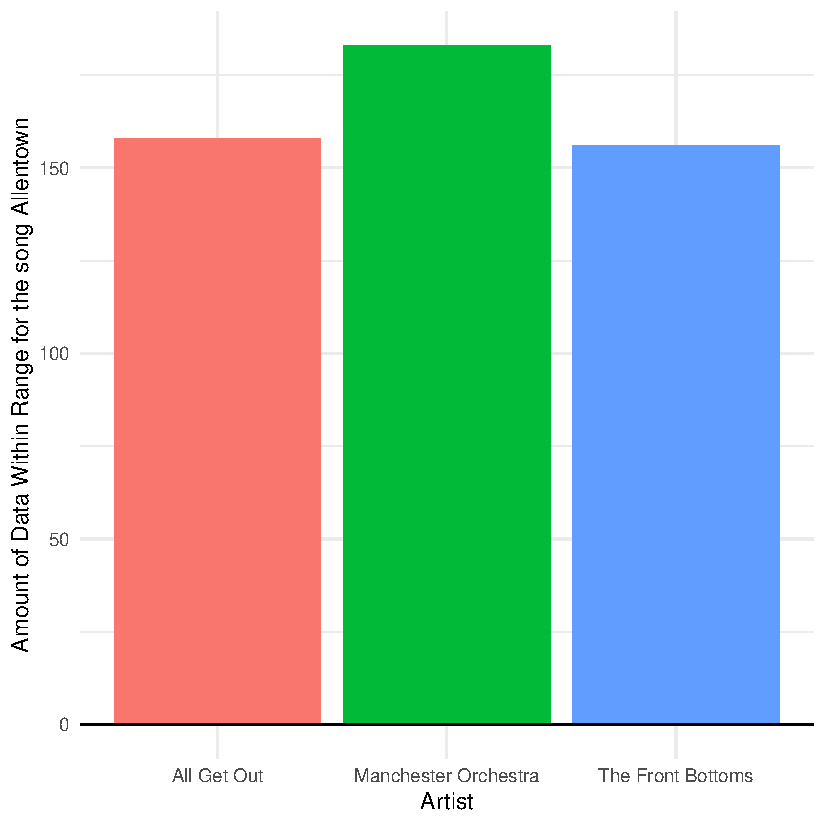
\includegraphics[width=\maxwidth]{figure/unnamed-chunk-1-1} 
\end{knitrout}
\caption{Number of Statistics Within Range for Each Band}
\label{Figure 1}
\end{center}
\end{figure}


\begin{figure}[ht]
\begin{center}
\begin{knitrout}
\definecolor{shadecolor}{rgb}{0.969, 0.969, 0.969}\color{fgcolor}
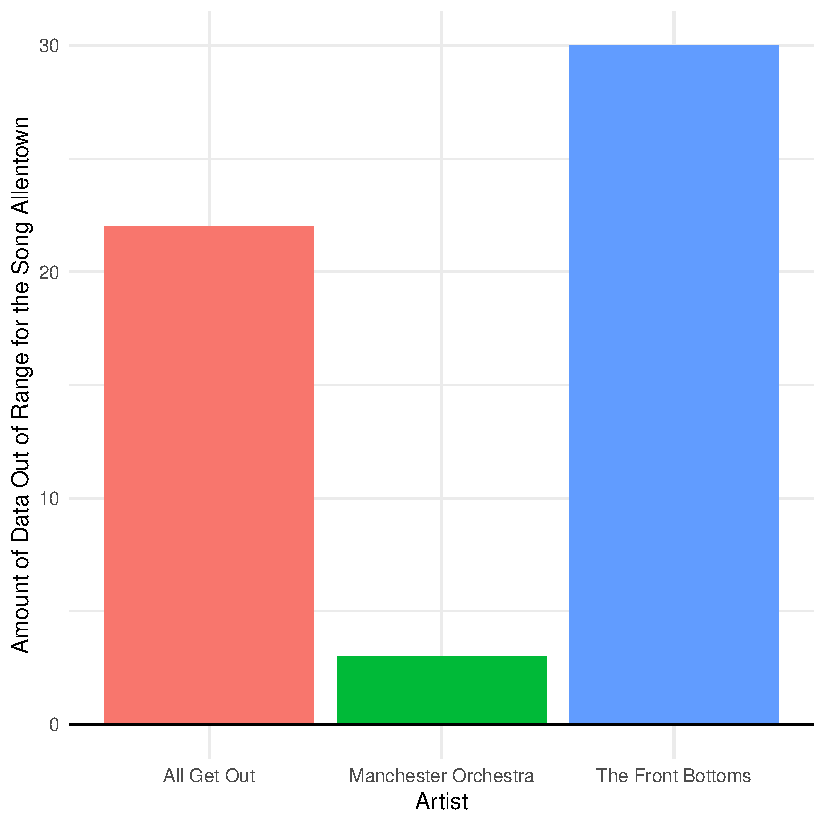
\includegraphics[width=\maxwidth]{figure/unnamed-chunk-2-1} 
\end{knitrout}
\caption{Number of Statistics Out of Range for Each Band}
\label{Figure 2}
\end{center}
\end{figure}
\begin{figure}[ht]
\begin{center}
\begin{knitrout}
\definecolor{shadecolor}{rgb}{0.969, 0.969, 0.969}\color{fgcolor}
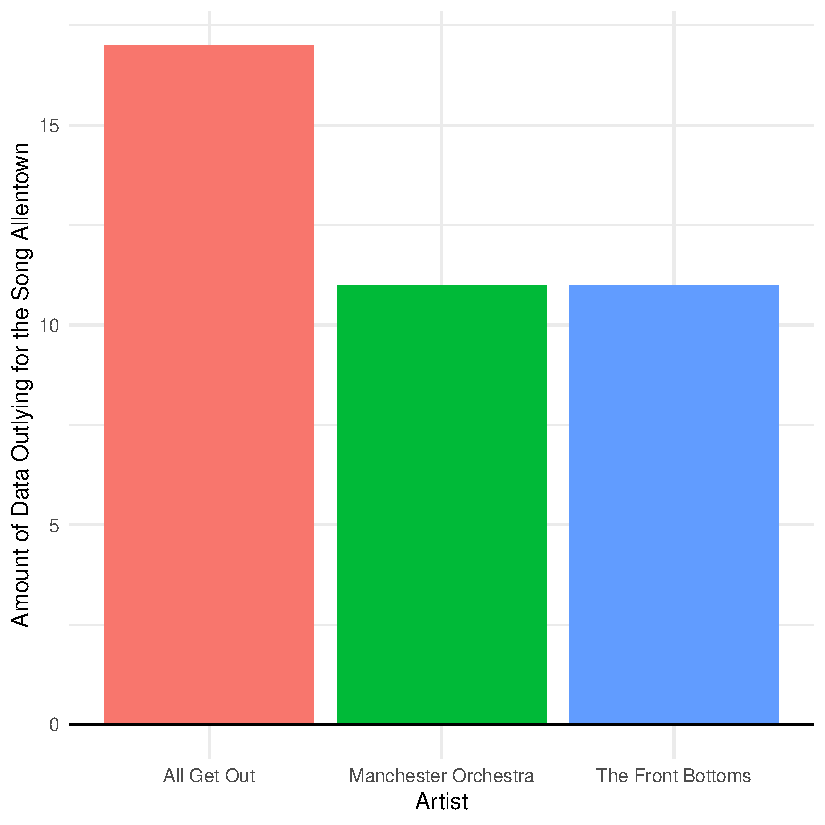
\includegraphics[width=\maxwidth]{figure/unnamed-chunk-3-1} 
\end{knitrout}
\caption{Number of Statistics Outlying for Each Band}
\label{Figure 3}
\end{center}
\end{figure}







\end{document}



